\documentclass{beamer}
\usepackage[utf8]{inputenc}

\usetheme{Madrid}
\usecolortheme{default}
\usepackage{amsmath,amssymb,amsfonts,amsthm}
\usepackage{txfonts}
\usepackage{tkz-euclide}
\usepackage{listings}
\usepackage{adjustbox}
\usepackage{array}
\usepackage{tabularx}
\usepackage{gvv}
\usepackage{lmodern}
\usepackage{circuitikz}
\usepackage{tikz}
\usepackage{graphicx}

\setbeamertemplate{page number in head/foot}[totalframenumber]

\usepackage{tcolorbox}
\tcbuselibrary{minted,breakable,xparse,skins}



\definecolor{bg}{gray}{0.95}
\DeclareTCBListing{mintedbox}{O{}m!O{}}{%
  breakable=true,
  listing engine=minted,
  listing only,
  minted language=#2,
  minted style=default,
  minted options={%
    linenos,
    gobble=0,
    breaklines=true,
    breakafter=,,
    fontsize=\small,
    numbersep=8pt,
    #1},
  boxsep=0pt,
  left skip=0pt,
  right skip=0pt,
  left=25pt,
  right=0pt,
  top=3pt,
  bottom=3pt,
  arc=5pt,
  leftrule=0pt,
  rightrule=0pt,
  bottomrule=2pt,

  colback=bg,
  colframe=orange!70,
  enhanced,
  overlay={%
    \begin{tcbclipinterior}
    \fill[orange!20!white] (frame.south west) rectangle ([xshift=20pt]frame.north west);
    \end{tcbclipinterior}},
  #3,
}
\lstset{
    language=C,
    basicstyle=\ttfamily\small,
    keywordstyle=\color{blue},
    stringstyle=\color{orange},
    commentstyle=\color{green!60!black},
    numbers=left,
    numberstyle=\tiny\color{gray},
    breaklines=true,
    showstringspaces=false,
}
%------------------------------------------------------------
%This block of code defines the information to appear in the
%Title page
\title %optional
{4.13.33}
\date{October - 2025}
%\subtitle{A short story}

\author % (optional)
{J.NAVYASRI- EE25BTECH11028}

\begin{document}

\frame{\titlepage}
\begin{frame}{Question:}
    Find the locus of a variable point \(\myvec{P} = \myvec{(x, y)}\) whose distance from the point \(\myvec{A} = \myvec{(-2, 0)}\) is 
\(\dfrac{2}{3}\) times its distance from the line \(x = -\dfrac{9}{2}\).
\end{frame}


\begin{frame}{Solution:}
Let
\[
\myvec{x}=\myvec{x\\[4pt]y},\qquad
\myvec{a}=\myvec{-2\\[4pt]0},\qquad
\myvec{n}=\myvec{1\\[4pt]0},\qquad
c=\frac{9}{2}.
\]

Distance condition (given):
\begin{equation}
\label{eq:dist}
\left\lVert \myvec{x}-\myvec{a} \right\rVert
= \frac{2}{3}\,\big|\myvec{n}^T\myvec{x}+c\big|.
\end{equation}

Square both sides:
\begin{equation}
\label{eq:squared}
(\myvec{x}-\myvec{a})^T(\myvec{x}-\myvec{a})
= \frac{4}{9}\big(\myvec{n}^T\myvec{x}+c\big)^2.
\end{equation}
\end{frame}

\begin{frame}{Solution:}
Evaluate each side in coordinates:
\begin{align}
(x+2)^2 + y^2
&= \frac{4}{9}\!\left(x+\frac{9}{2}\right)^{\!2} \\
x^2+4x+4 + y^2
&= \frac{4}{9}x^2 + 4x + 9 \\
\text{(cancel }4x\text{ on both sides)}\qquad
x^2 + 4 + y^2
&= \frac{4}{9}x^2 + 9
\end{align}
\end{frame}

\begin{frame}{Solution:}

Multiply both sides by $9$:
\[
9x^2 + 36 + 9y^2 = 4x^2 + 81
\]
\[
\Rightarrow 5x^2 + 9y^2 = 45.
\]

Divide by $45$ to get standard form:
\begin{equation}
\boxed{\;\dfrac{x^2}{9} + \dfrac{y^2}{5} = 1\;}
\end{equation}

Thus the locus is an ellipse centered at the origin with semi-axes $3$ (along $x$) and $\sqrt{5}$ (along $y$).
\end{frame}



\begin{frame}[fragile]
    \frametitle{Python Code}
    \begin{lstlisting}
import numpy as np
import matplotlib.pyplot as plt

# Define theta
theta = np.linspace(0, 2*np.pi, 400)

# Ellipse parameters
a = 3  # semi-major axis
b = np.sqrt(5)  # semi-minor axis

x = a * np.cos(theta)
y = b * np.sin(theta)
\end{lstlisting}
\end{frame}


\begin{frame}[fragile]
    \frametitle{Python Code}
    \begin{lstlisting}
plt.plot(x, y, label=r'$\dfrac{x^2}{9} + \dfrac{y^2}{5} = 1$')

plt.xlabel("x-axis")
plt.ylabel("y-axis")
plt.title("Ellipse Locus")
plt.grid(True)

# Move legend to top-right
plt.legend(loc="upper right")

plt.axis("equal") 
plt.savefig("fig9.png") 
plt.show()
\end{lstlisting}
\end{frame}

\begin{frame}[fragile]
    \frametitle{ C Code}
    \begin{lstlisting}
#include <stdio.h>
#include <math.h>

int main() {
    FILE *fp = fopen("ellipse.dat", "w");
    if (fp == NULL) {
        printf("Error opening file!\n");
        return 1;
    }
\end{lstlisting}
\end{frame}

\begin{frame}[fragile]
    \frametitle{ C Code}
    \begin{lstlisting}
    double a = 3.0;          // semi-major axis (x-direction)
    double b = sqrt(5.0);    // semi-minor axis (y-direction)
    double theta;

    for (theta = 0; theta <= 2*M_PI; theta += 0.01) {
        double x = a * cos(theta);
        double y = b * sin(theta);
        fprintf(fp, "%lf %lf\n", x, y);
    }

    fclose(fp);
    printf("Data written to ellipse.dat\n");
    printf("Use: gnuplot -e \"plot 'ellipse.dat' with lines title 'x^2/9 + y^2/5 = 1'\"\n");
    return 0;
}
\end{lstlisting}
\end{frame}


\begin{frame}[fragile]
    \frametitle{Python and C code}
    \begin{lstlisting}

import ctypes
import numpy as np
import matplotlib.pyplot as plt

# Load compiled C library
lib = ctypes.CDLL("./libellipse.so")

# Define argument and return types
lib.ellipse_point.argtypes = [ctypes.c_double, ctypes.c_double,
                              ctypes.c_double,
                              ctypes.POINTER(ctypes.c_double),
                              ctypes.POINTER(ctypes.c_double)]

# Semi-axes
a = 3.0
b = np.sqrt(5.0)
\end{lstlisting}
\end{frame}


\begin{frame}[fragile]
    \frametitle{Python and C  Code}
    \begin{lstlisting}
# Generate ellipse points
theta_vals = np.linspace(0, 2*np.pi, 400)
x_vals, y_vals = [], []

for theta in theta_vals:
    x = ctypes.c_double()
    y = ctypes.c_double()
    lib.ellipse_point(a, b, theta, ctypes.byref(x), ctypes.byref(y))
    x_vals.append(x.value)
    y_vals.append(y.value)
\end{lstlisting}
\end{frame}


\begin{frame}[fragile]
    \frametitle{Python and C code}
    \begin{lstlisting}
# Plot ellipse
plt.plot(x_vals, y_vals, label=r'$\dfrac{x^2}{9} + \dfrac{y^2}{5} = 1$')
plt.xlabel("x-axis")
plt.ylabel("y-axis")
plt.title("Ellipse Locus")
plt.grid(True)
plt.legend(loc="upper right")
plt.axis("equal")
plt.show()
\end{lstlisting}
\end{frame}
\begin{frame}{Plot-Using Python}
    \centering
    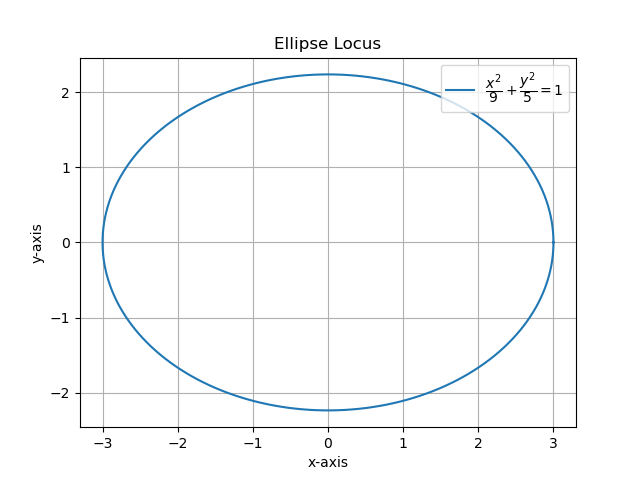
\includegraphics[width=\columnwidth, height=0.8\textheight, keepaspectratio]{figs/fig9.png}     
\end{frame}
\end{document}

